\chapter{真题讲解}
\label{chap23}

%杭电真题只有近三年的价值最高,其他的如果时间不足可以不做☆ \newline
%对应2020年考研,2017,2018,2019三年最为重要.\newline
%因为有一些题目出的模棱两可,实在不必深究,这种题目会越来越少,越来越逼近408这就是趋势。\newline
%注解:QU 表示此题有疑问\newline
\begin{comment}


\begin{itemize}[noitemsep,topsep=0pt,parsep=0pt,partopsep=0pt]
	\item 2019数据结构和组成原理真题(150分)
	\item 2019数据结构和组成原理真题答案
\end{itemize}


\section{杭州电子科技大学2019年攻读硕士学位研究生招生考试《数据结构与组成原理》试题}
(试题共9大题,共10页,总分150分)\newline
姓名\_\_\_\_ 报考专业\_\_\_\_ 准考证号\_\_\_\_\newline
【所有答案必须卸载答题纸上,做在试卷或草稿纸上无效!】\newline
\subsection{一、单向选择题(本大题共7小题,每小题2分,本大题共14分)}
1. 为解决计算机主机与打印机之间速度不匹配问题,通常设置一个打印数据缓冲区,主机将要输出的数据依次写入该缓冲区,而打印机则依次从该缓冲区中取出数据。该缓冲区的逻辑结构应该是( )。\newline
A. 栈  B. 队列   C. 树  D. 图\newline
2. 已知操作符包括‘+’、‘-’、‘*’、‘/’、‘(’,‘)’。将中缀表达式 a+b=a*((c+d)/e - f)+g转换为等价的后缀表达式ab+acd+e/f-*-g+时,用栈来存放暂时还不能确定运算次序的操作符,若栈初始时为空,则转换过程中同时保存在栈中的操作符的最大个数是( ).\newline
A. 5   B. 7  C. 8 D. 11\newline
3. 在一棵度为4的树T中,若有20个度为4的节点,10个度为3的节点,1个度为2的节点,10个度为1的节点,若树T的叶结点个数树( ).\newline
A.41   B.82    C.113   D.12\newline
4. 在任意一棵非空二叉排序树T1中,删除某个节点v之后形成二叉排序树T2,再将v插入T2形成二叉排序树T3。下列关于T1和T3的叙述中,正确的是( ).\newline
\uppercase\expandafter{\romannumeral1}. 若v是T1的叶节点,则T与T3不同\newline
\uppercase\expandafter{\romannumeral2}. 若v是T1的叶节点,则T与T3相同\newline
\uppercase\expandafter{\romannumeral3}. 若v不是T1的叶节点,则T1与T3不同\newline
\uppercase\expandafter{\romannumeral3}. 若v不是T1的叶节点,则T1与T3相同\newline
A. 仅\uppercase\expandafter{\romannumeral1}、\uppercase\expandafter{\romannumeral3} B. 仅\uppercase\expandafter{\romannumeral1}、\uppercase\expandafter{\romannumeral4} C.  仅\uppercase\expandafter{\romannumeral2}、\uppercase\expandafter{\romannumeral3} D.  仅\uppercase\expandafter{\romannumeral2}、\uppercase\expandafter{\romannumeral4} \newline
5. 循环队列放在一维数组A[0...M-1]中,end1指向队头元素,end2指向队尾元素的后一个位置。假设队列两端均可进行入队和出队操作,队列中最多能容纳M-1个元素。初始时为空。下列判断队空和队满的条件中,正确的是( )。\newline
A. 队空:end1 == end2; 队满: end1 == (end2 + 1)mod M\newline
B. 队空:end1 == end2; 队满: end2 == (end1 + 1)mod(M-1) \newline
C. 队空:end2 == (end1+1)mod M; 队满: end1 == (end2+1)mod M \newline
D. 队空:end1 == (end2+1)mod M; 队满:end2 == (end1 + 1)mod (M-1) \newline
6. 有一个100阶的三对角矩阵 M, 其元素$m_{i,j}(1\le i \le 100, 1 \le j \le 100)$按行优先次序压缩存入下标从0开始的一维数组N中。元素$m_{30,30}$在N中的小标是(  ).\newline
A. 86 B. 87 C.88 D. 89 \newline
7. 键字序列 5, 8, 12, 19, 28, 20, 15, 22 是小根堆(最小堆),插入关键字3,调整后得到的小根堆是( ).\newline
A. 3, 5, 12, 8, 28, 20, 15, 22, 19\newline
B. 3, 5, 12, 19, 20, 15, 22, 8, 28\newline
C. 3, 8, 12, 5, 20, 15, 22, 28, 19\newline
D. 3, 12, 5, 8, 28, 20, 15, 22, 19\newline
\subsection{二、填空题 (本大题共7空,每空2分,本大题共14分)}
1. 已知指针P指向单链表L中的某节点,则删除其后继节点的语句是:\_\_\_.\newline
2. 设广义表(((a,b), x),((a),(b)),(c,(d,(y)))), 得到y的对广义表A的操作序列是:\_\_\_.\newline
3. 已知一棵树有2011个节点的树,其叶节点个数为116,该树对应的二叉树中无右孩子的节点个数是:\_\_\_.\newline
4. 有向图G=(V,E),其中V(G)={0,1,2,3,4,5}, 用<a,b,d>三元组表示弧<a,b>及弧上的权d. E(G)={<0,5,100>, <0,2,10>, <1,2,5>, <0,4,30>, <4,5,60>, <3,5,10>, <2,3,50>, <4,3,20>}, 则从源点0到顶点3的最短路径长度是\_\_\_,经过的中间顶点是\_\_\_.\newline
5. 127阶B-树种每个节点最多有\_\_\_个关键字; 除根节点外外所有非终端节点至少有\_\_\_棵子树。\newline
\subsection{三、简答题(本大题共4小题,每小题10分,本大题共40分)}
1. 将关键字序列(7、 8、 30、 11、 18、 9、 14)散列存储到散列表中。散列表存储空间是一个下标从0开始的一维数组,散列函数为:H(key) = (key*3)MOD7,处理冲突采用线性探测再散列法,要求装填(载)因子为0.7.\newline
(1) 请画出所构造的散列表。\newline
(2) 分别计算等概率情况下查找成功和查找失败的平均查找长度。\newline
2. 假定有系列n*n矩阵(n为奇数)\newline
\begin{figure}[H]
	\centering  % 环境中的内容居中排版
	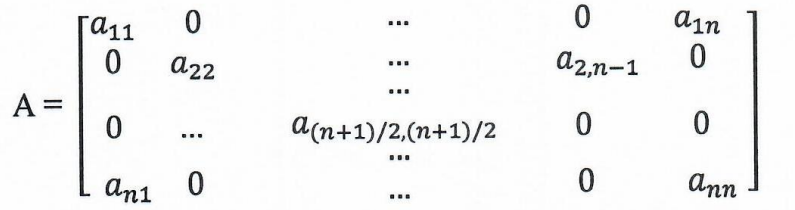
\includegraphics[scale=0.3]{example/chapter23/Annotation2019-09-21142808.png}
\end{figure}
如果用一维数组B按行主次序存储A的非零元素,问:\newline
(1) A 中 非零元素的行下标与列下标的关系;\newline
(2) 给出A中非零元素$a_{i,j}$的小标(i,j)与B中的下标R的关系;\newline
(3) 假定矩阵中每个元素占一个存储单元且B的起始地址为$A_0$,给出利用$a_{i,j}$的下标定位在B中的位置公式.\newline
3. 对下面的3阶B-树,一次执行下列操作,画出各步操作的结果。\newline
\begin{figure}[H]
	\centering  % 环境中的内容居中排版
	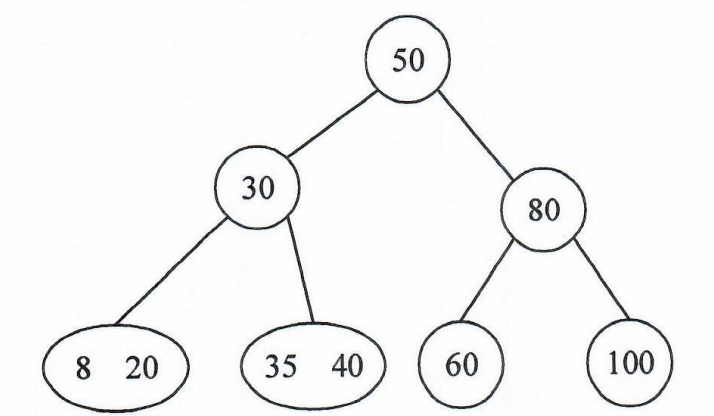
\includegraphics[scale=0.3]{example/chapter23/Annotation2019-09-21144459.png}
\end{figure}
(1) 插入 90  (2) 插入25 (3) 插入45 (4) 删除60 (5)删除 80\newline
4. 下标给出了某工程各工序之间的优先关系和各工序所需时间.\newline
\begin{figure}[H]
	\centering  % 环境中的内容居中排版
	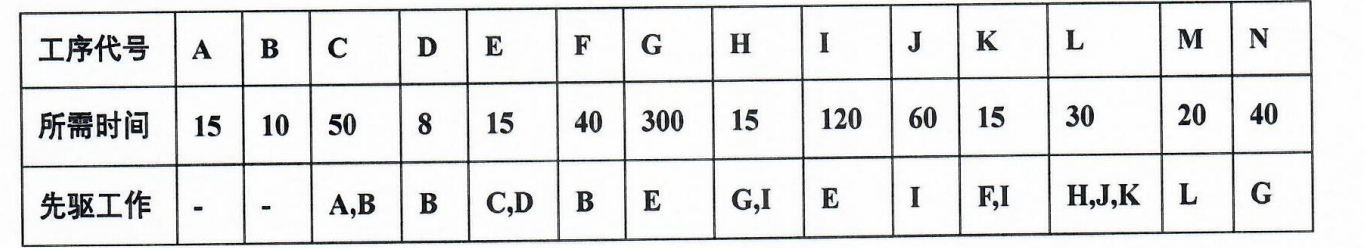
\includegraphics[scale=0.3]{example/chapter23/Annotation2019-09-21144810.png}
\end{figure}
(1) 画出相应的AOE网;\newline
(2) 列出各时间的最早发生时间,最迟发生时间;\newline
(3) 找出关键路径并指明完成该工程所需最短时间.\newline
\subsection{四、程序阅读题(本大题共3小题, 每小题5分, 本大题共15分)}
1. 算法一:\newline
\begin{lstlisting}[basicstyle=\small\ttfamily, caption={}, numbers=none]
int con(graph g){
	int i, flag = 1;
	int visited[Vnum];
	for(i=0; i<g.vexnum; i++)
		visited[i] = 0;
	dfs(g, 0, visited);
	for(i=0; i<g.vexnum; i++)
		if( visited[i] == 0 ){
			flag = 0; 
			break;
		}
	return flag;
}
\end{lstlisting}

2. 算法二:\newline
\begin{lstlisting}[basicstyle=\small\ttfamily, caption={}, numbers=none]
int com(int A[], int \&a, int B[], int nb){
	if(na + nb > maxSize)
		return -1;
	int i=na, j = nb;
	while(j>0){
		if(i==0||A[i-1]<B[j-1]){
			A[j+i-1] = B[j-1];
			--j; 
		}else{
			A[j+i-1] = A[i-1];
			--i;
		}
	}
	na = na + nb;
	return na;
}
\end{lstlisting}

3. 算法三:\newline
\begin{lstlisting}[basicstyle=\small\ttfamily, caption={}, numbers=none]
void cop(int a[], int n){
	change=1;low=0;high=n-1;
	while(low<high && change){
		change=0;
		for(i=low; i<high; i++){
			if(a[i] > a[i+1]){
				a[i] <--> a[i+1];
				change=1;
			}
		}
		high--;
		for(i=high; i>low; i--){
			if(a[i]>a[i-1]){
				a[i]<-->a[i-1];
				change=1;
			}
		}
		low++;
	}
}
\end{lstlisting}

\subsection{五、算法设计题(本大题共2小题,每小题11分, 本大题共22分)}
1. 已知两个无表头及诶按的单链表p1及单链表p2,分别表示两个多项式。链表中的一个节点对应多项式中的一个单项,每个单项节点包含两个数据域,分别表示单项的系数和指针;一个指针域,指向下一个单项节点。\newline
\begin{lstlisting}[basicstyle=\small\ttfamily, caption={}, numbers=none]
struct PolyNode{
	int coef;
	int expon;
	struct PolyNode *link;
};
typedef struct PolyNode* Polynomial;
\end{lstlisting}
p1 和 p2 中的节点按照单项的指数递减排列。写一个算法,实现p1和p2相加,并将计算结果存入新的无表头节点的单链表中。\newline
2.给定两棵二叉树T1和T2,若T1可以通过若干次左右孩子交换变成T2,则称T1和T2是"同构"的。已知有静态链表表示的两棵二叉树T1、T2(T1和T2分别为两棵二傻叔根节点的编号),写一个算法,判断给定的两棵二叉树是否同构。(注:静态链表是指有数组表示的二叉树,数组中的第i个元素对应二叉树中编号为i的节点。并且,每个元素包含三个数据域:节点的关键字值、节点左孩子节点的编号和节点有孩子节点的编号,若某个节点无孩子,则其孩子节点编号为-1).\newline
\begin{figure}[H]
	\centering  % 环境中的内容居中排版
	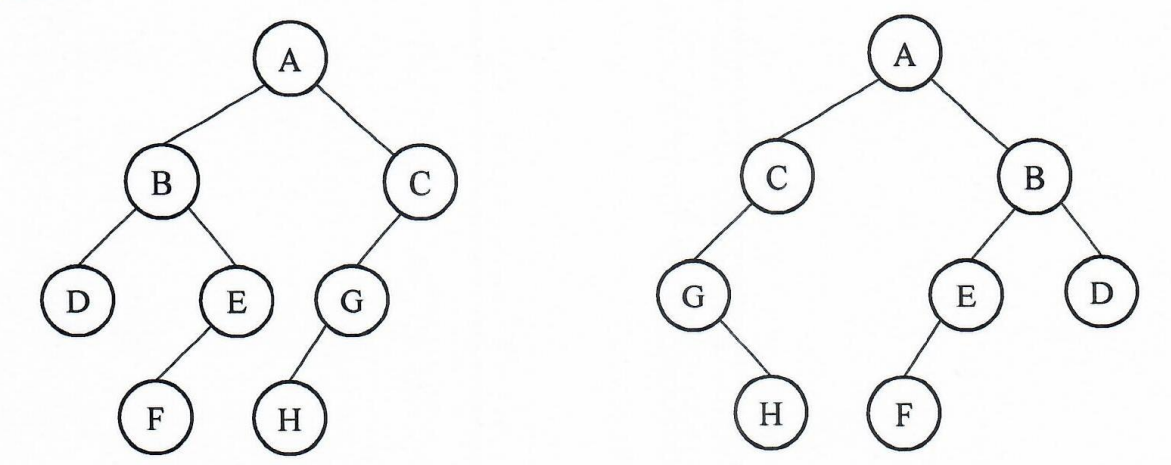
\includegraphics[scale=0.3]{example/chapter23/Annotation2019-09-21202832.png}
\end{figure}
\begin{lstlisting}[basicstyle=\small\ttfamily, caption={}, numbers=none]
#define MaxTree 10
#define ElementType char
#define Tree int
#define Null -1
struct TreeNode{
	ElementType Element;
	Tree Left;
	Tree Right;
}T1[MaxTree],T2[MaxTree];
\end{lstlisting}
\subsection{六、计算题(本大题共3小题,本大题共10分)}
设浮点数的格式为:阶码6bit,包含1bit符号,用移码表示。位数10bit,包含1bit符号,用补码表示。浮点数排列顺序为:\newline
\begin{tabular}{|c|c|c|c|}% 通过添加 | 来表示是否需要绘制竖线
	\hline  % 在表格最上方绘制横线
	阶符(1bit) & 阶码(5bit) & 数符(1bit) & 尾数(9bit) \\
	\hline % 在表格最下方绘制横线
\end{tabular}
1.(本小题2分)若$(X)_{10} = 13/64$,则按上述浮点数的格式,写出X的规格化浮点数表示形式。\newline
2.(本小题2分)该浮点数格式(非规格化)可表示的数据的精度是多少?\newline
3.(本小题6分)设浮点数$[X]_{\mbox{浮}}$和$[Y]_{\mbox{浮}}$分别以大端模式存储在地址10H和12H开始连续的存储单元中,如表1所示:\newline
表1 浮点数X和Y的存储格式\newline
\begin{tabular}{|c|c|}% 通过添加 | 来表示是否需要绘制竖线
	\hline  % 在表格最上方绘制横线
	地址 & 存储单元内容 \\
	\hline % 在表格最下方绘制横线
	10H & FDH \\
	\hline % 在表格最下方绘制横线
	11H & 50H \\
	\hline % 在表格最下方绘制横线
	12H & FAH \\
	\hline % 在表格最下方绘制横线
	13H & A0H \\
	\hline % 在表格最下方绘制横线
\end{tabular}\newline
求$[X-Y]_{\mbox{浮}}$。(要求阶码用移码计算,尾数用补码计算,结果规格化表示,写出计算过程、步骤等)\newline
\subsection{七、设计题(本大题共2小题,本大题共10分)}
1.(本小题6分)设CPU地址线有$A_{15}~A_{0}$,数据线有$D_7 ~ D_0$,读写信号线$\bar{WE}$(低电平写,高电平度),存储器请求线$\bar{MREQ}$(低电平有效),CPU与2片8K$\times$8bit的ROM和1片8k$\times$16bit的SRAM组成的32K$times$8bit的存储器系统,OE\#为输出允许信号(低电平有效),$\bar{CS}$为芯片选择信号(低电平于晓),R/$\bar{W}$为读写信号(高电平为度,低电平为写),其中ROM的地址从2000H开始占有16K连续地址空间,SRAM的地址从8000H开始占有连续的16K地址空间,指出下面图1CPU与存储器的链接途中的错误,并改正之。\newline
\begin{figure}[H]
	\centering  % 环境中的内容居中排版
	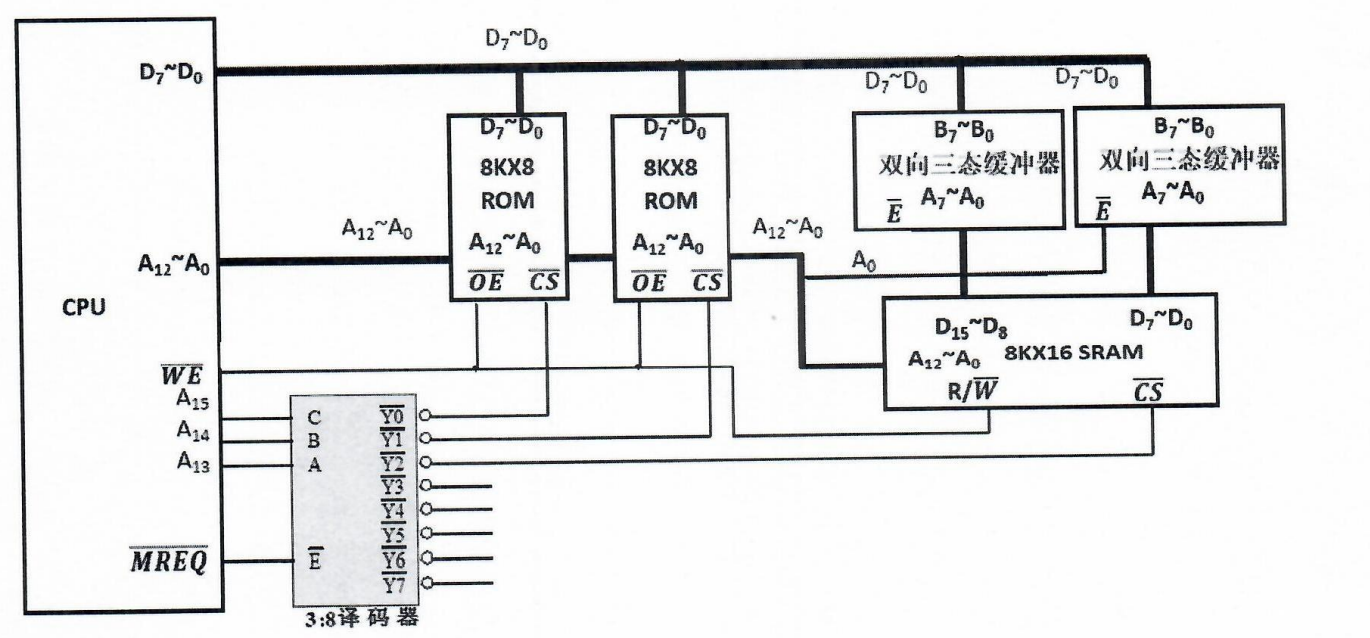
\includegraphics[scale=0.3]{example/chapter23/Annotation2019-09-21205443.png}
\end{figure}
2. (本小题4分)设CPU字长为32bit,存储器按字节编址,用256KB存储器芯片组成一个1M*32bit的存储器系统,若存储周期T=200ns,总线传输周期为50ns,存储器系统如何组织才能最大地限度地提高存储器带宽?并请画出主存地址字段组织格式(即请写出字段中低位地址的作用和尾数,高位的地址的作用和位数).\newline
\subsection{八、(本大题共10分)} 
设下列程序中的指令均为双字节指令,个数如下:\newline
\begin{center}

\begin{tabular}{|c|c|c|}% 通过添加 | 来表示是否需要绘制竖线
	\hline  % 在表格最上方绘制横线
	指令操作码(4bit) & 源操作数寻址方式(2bit) & 目的寄存器地址(2bit) \\
	\hline % 在表格最下方绘制横线
	\multicolumn{3}{c|}{Imm/Addr/Disp}\\
	\hline
\end{tabular}
\end{center}
指令的第二自己含义与指令相关,可以是8bit立即数、或是8bit地址、或是8bit偏移量,存储器按自己编织,即CPU每次只能从存储器读取或写入一个字节,设该程序从内存地址00h开始装入,R0~R3分别为4个寄存器,R2也可以作为变址寄存器使用。\newline
\begin{lstlisting}[basicstyle=\small\ttfamily, caption={}, numbers=none]
start:  MOV R0, #40H ; 数据 40H -> R0
		MOV R1, #10  ; 数据10-> R1
		MOV R2, #0   ; 清0R2
LOOP:	ADD R0, [R2 + 2] ; (R0) +[(R2) + 10]->R0,
		ADD R2, #1       ; (R2) + 1 -> R2
		SUB R1, #1       ; (R1) -1 -> R1
		JNZ LOOP         ; 结果非0转loop处执行,相对寻址
		HALT             ; 停机
\end{lstlisting}
请问:\newline
1. (本小题2分) 相对转移指令JNZ LOOP 的8位二进制偏移量等于多少?\newline
2. (本小题2分) 指令ADD R0,[R2+10]的源操作数曹勇的是何种寻址方式?\newline
3. (本小题3分) 若系统有一容量为8字节的cache,采用2路组相联映射,每块2字节。设cache在执行该程序前为空,则执行完这段程序,cache的命中率为多少?\newline
4. (本小题3分) 第4小题中,设访问存储器的时间需100ns,访问cache的时间为10ns,若CPU总是从Cache中访问数据,则执行这段程序所需的时间等于多少??\newline
\subsection{九、(本大题共15分)}
设MIPS单周期CPU结构和数据通路如图2所示,数据流动方向由箭头所示,图中的三个二选一电路的控制信号定于如表2所示,指令各字段含义如下:\newline
OP:操作码,func:指令的功能码,imm:指令中的16bit的立即数,rt:寄存器rt地址,rd:寄存器rd地址;寄存器和存储器字长都是32bit,R\_Addr\_A,R\_Addr\_B分别是寄存器堆的二个读端口地址输入端,W\_Addr是寄存器堆的写端口地址输入端,W\_Data是寄存器堆的写输入输入端口,R\_Data\_A和R\_Data\_B分别是寄存器堆的二个数据输出端,图2中二选一电路选择信号和部分指令译码输出的控制信号的取值定义如表2所示.\newline
\begin{figure}[H]
	\centering  % 环境中的内容居中排版
	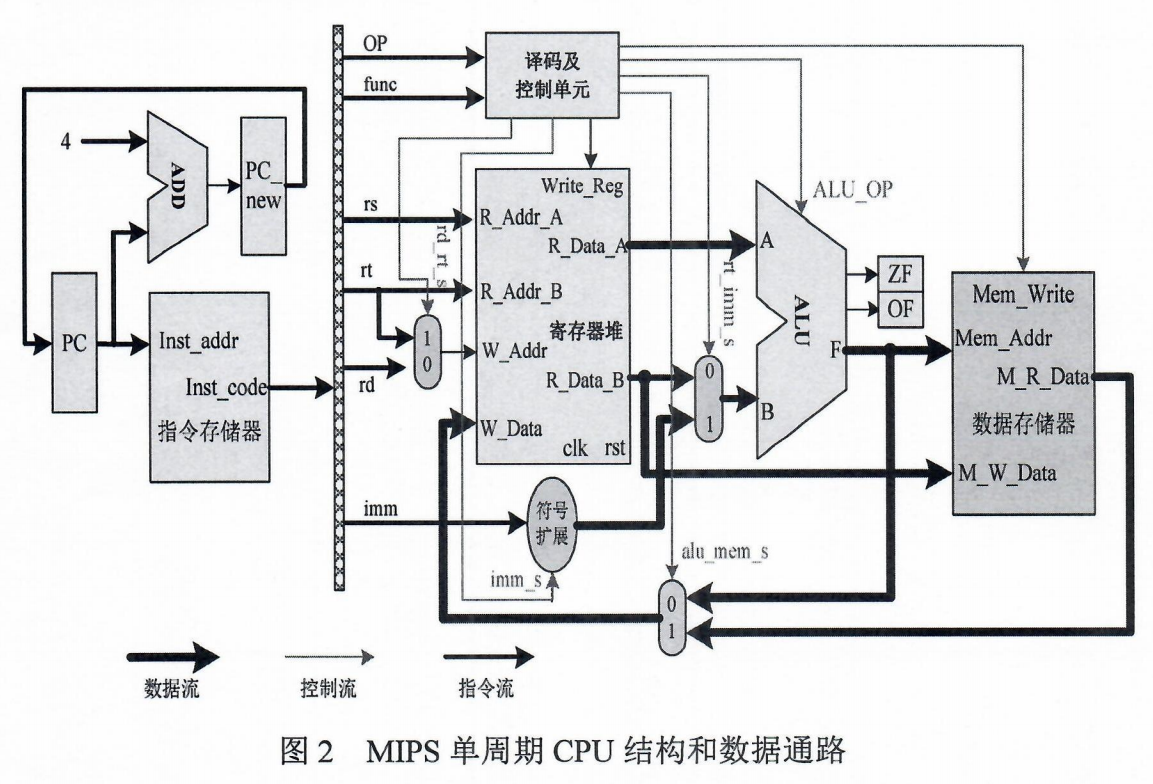
\includegraphics[scale=0.3]{example/chapter23/Annotation2019-09-28124114.png}
\end{figure}
\begin{figure}[H]
	\centering  % 环境中的内容居中排版
	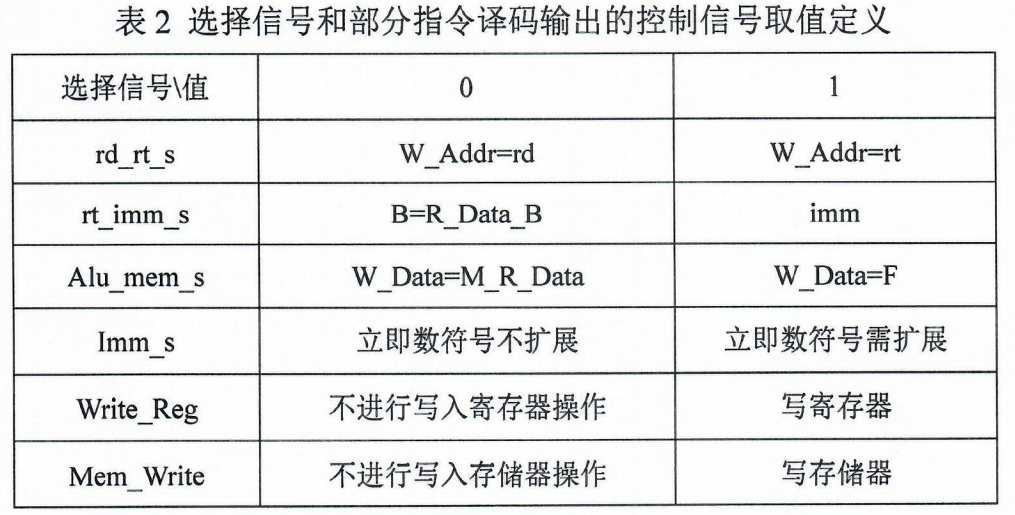
\includegraphics[scale=0.3]{example/chapter23/Annotation2019-09-28124147.png}
\end{figure}
若执行指令:ANDi rt, rs, imm; 位与:(rs)\&imm->rt\newline
1. (本小题6分) 写出当执行该指令是的数据通路对应的控制信号状态值填入表3中。\newline
\begin{figure}[H]
	\centering  % 环境中的内容居中排版
	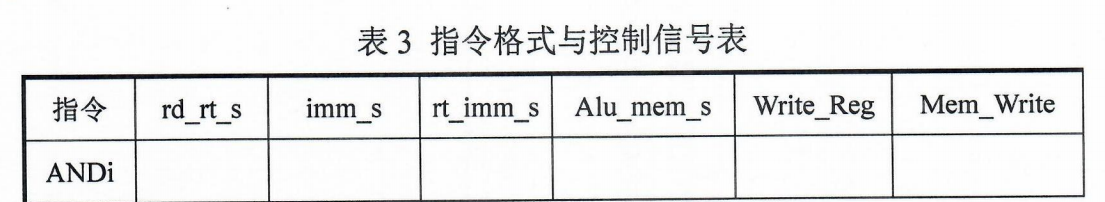
\includegraphics[scale=0.3]{example/chapter23/Annotation2019-09-28124513.png}
\end{figure}
2. (本小题2分) 请解释在图2中,为什么指令从指令存储器读出后,是直接保持在指令总线上而不需要指令寄存器IR来存放指令?\newline
3. (本小题2分) 图2的CPU结构能否实现相对转移指令JNZ rel?为什么?\newline
4. (本小题2分) 设指令中的16bit立即数分别为79FBH和9F69H,则经过符号位扩展后得到的32bit数据分别应为多少?\newline
5. (本小题2分) 图2的体系结构是哈弗结构还是普林斯顿结构?每执行一条指令PC寄存器的值加了多少? \newline
6. (本小题1分) 图2从系统结构来看,属于SISD,SIMD,MISD,MIMD四种结构的哪一种?\newline

\end{comment}



\section{杭州电子科技大学2019年计算机考研真题答案}

\subsection{一、单向选择题(本大题共7小题,每小题2分,本大题共14分)}
1.\newline
B \newline 
略\newline
2.\newline
A \newline
栈中数据 1) +  2) - 3) -*(( 4) -*((+ 5) -*(/ \newline
输出数据 1) ab 2) + 3) a    4) cd    5) +e   后面就开始减少了所以最多个数是5 \newline
3.\newline
B \newline
公式 结点和分支的关系 结点数 - 1 == 分支数\newline
20 + 10 + 1 + 10 + x -1 = 20*4 + 10 *3 + 1 * 2 + 10 * 1\newline
x = 82\newline
4.\newline
C \newline
略\newline
5.\newline
A \newline
front 和 rear 之间空一个元素作为判断满还是空\newline
6. \newline
B\newline
略\newline
7. \newline
A \newline
画出小根堆,然后把3放入最后面,然后重建小根堆即可\newline
\subsection{二、填空题 (本大题共7空,每空2分,本大题共14分)}
1. 已知指针P指向单链表L中的某节点,则删除其后继节点的语句是:if(p->next)\{q = p->next;p->next=p->next->next;free(q)\}.\newline
2. 设广义表(((a,b), x),((a),(b)),(c,(d,(y)))), 得到y的对广义表A的操作序列是:Head(Head(Tail(Head(Tail(Head(Tail(Tail(A)))))))).\newline
3. 已知一棵树有2011个节点的树,其叶节点个数为116,该树对应的二叉树中无右孩子的节点个数是:1896.\newline
4. 有向图G=(V,E),其中V(G)={0,1,2,3,4,5}, 用<a,b,d>三元组表示弧<a,b>及弧上的权d. E(G)={<0,5,100>, <0,2,10>, <1,2,5>, <0,4,30>, <4,5,60>, <3,5,10>, <2,3,50>, <4,3,20>}, 则从源点0到顶点3的最短路径长度是:50,经过的中间顶点是:4.\newline
5. 127阶B-树种每个节点最多有:126个关键字; 除根节点外外所有非终端节点至少有64棵子树。\newline
\subsection{三、简答题(本大题共4小题,每小题10分,本大题共40分)}
1. \newline
(1) 请画出所构造的散列表。\newline
解:\newline
$\because \alpha = 0.7 所以构造的表长度是 10$\newline
计算Hey(key)\newline
~\\
\begin{center}
\begin{tabular}{|c|c|c|c|c|c|c|}% 通过添加 | 来表示是否需要绘制竖线
	\hline  % 在表格最上方绘制横线
	7 & 8 & 30 & 11 & 18 & 9 & 14 \\
	\hline  %在第一行和第二行之间绘制横线
	0 & 3 & 6  & 5  & 5  & 6 & 0 \\
	\hline % 在表格最下方绘制横线
\end{tabular}
\end{center}
~\\
构造的散列表\newline
~\\
\begin{center}
\begin{tabular}{|c|c|c|c|c|c|c|c|c|c|c|}% 通过添加 | 来表示是否需要绘制竖线
	\hline  % 在表格最上方绘制横线
	地址   & 0 & 1 & 2 & 3 & 4 & 5  & 6 & 7 & 8 & 9\\
	\hline  %在第一行和第二行之间绘制横线
	关键字 & 7 & 14&   & 8 &   & 11 & 30& 18& 9 &  \\
	\hline % 在表格最下方绘制横线
\end{tabular}
\end{center}
~\\
(2) 分别计算等概率情况下查找成功和查找失败的平均查找长度。\newline
$ASL_{\mbox{查找成功}} = (1 + 2 + 1 + 1 + 1 + 3 + 3) / 7 = \frac{12}{7}$\newline
$ASL_{\mbox{查找失败}} = (3 + 2 + 1 + 2 + 1 + 5 + 4) / 7 = \frac{18}{7}$\newline
2. \newline
(1) A 中 非零元素的行下标与列下标的关系;\newline
解:\newline
i = j 或 i + j = n + 1\newline
(2) 给出A中非零元素$a_{i,j}$的下标(i,j)与B中的下标R的关系;\newline
\begin{equation}
R=\left\{
\begin{aligned}
2 \times (i - 1), i = j\\
2 \times (i - 1), i+j = n+1, i < j \\
2 \times (i - 1), i+j = n+1, i > j
\end{aligned}
\right.
\end{equation}
(3) 假定矩阵中每个元素占一个存储单元且B的起始地址为$A_0$,给出利用$a_{i,j}$的下标定位在B中的位置公式.\newline
\begin{equation}
Loc(a_{i,j})=\left\{
\begin{aligned}
2 \times (i - 1) \times size, i = j\\
2 \times (i - 1) \times size, i+j = n+1, i < j \\
2 \times (i - 1) \times size, i+j = n+1, i > j
\end{aligned}
\right.
\end{equation}
size 为一个存储单元的大小\newline
3. 
(1) 插入 90  (2) 插入25 (3) 插入45 (4) 删除60 (5)删除 80\newline
解:\newline
\begin{figure}[H]
	\centering  % 环境中的内容居中排版
	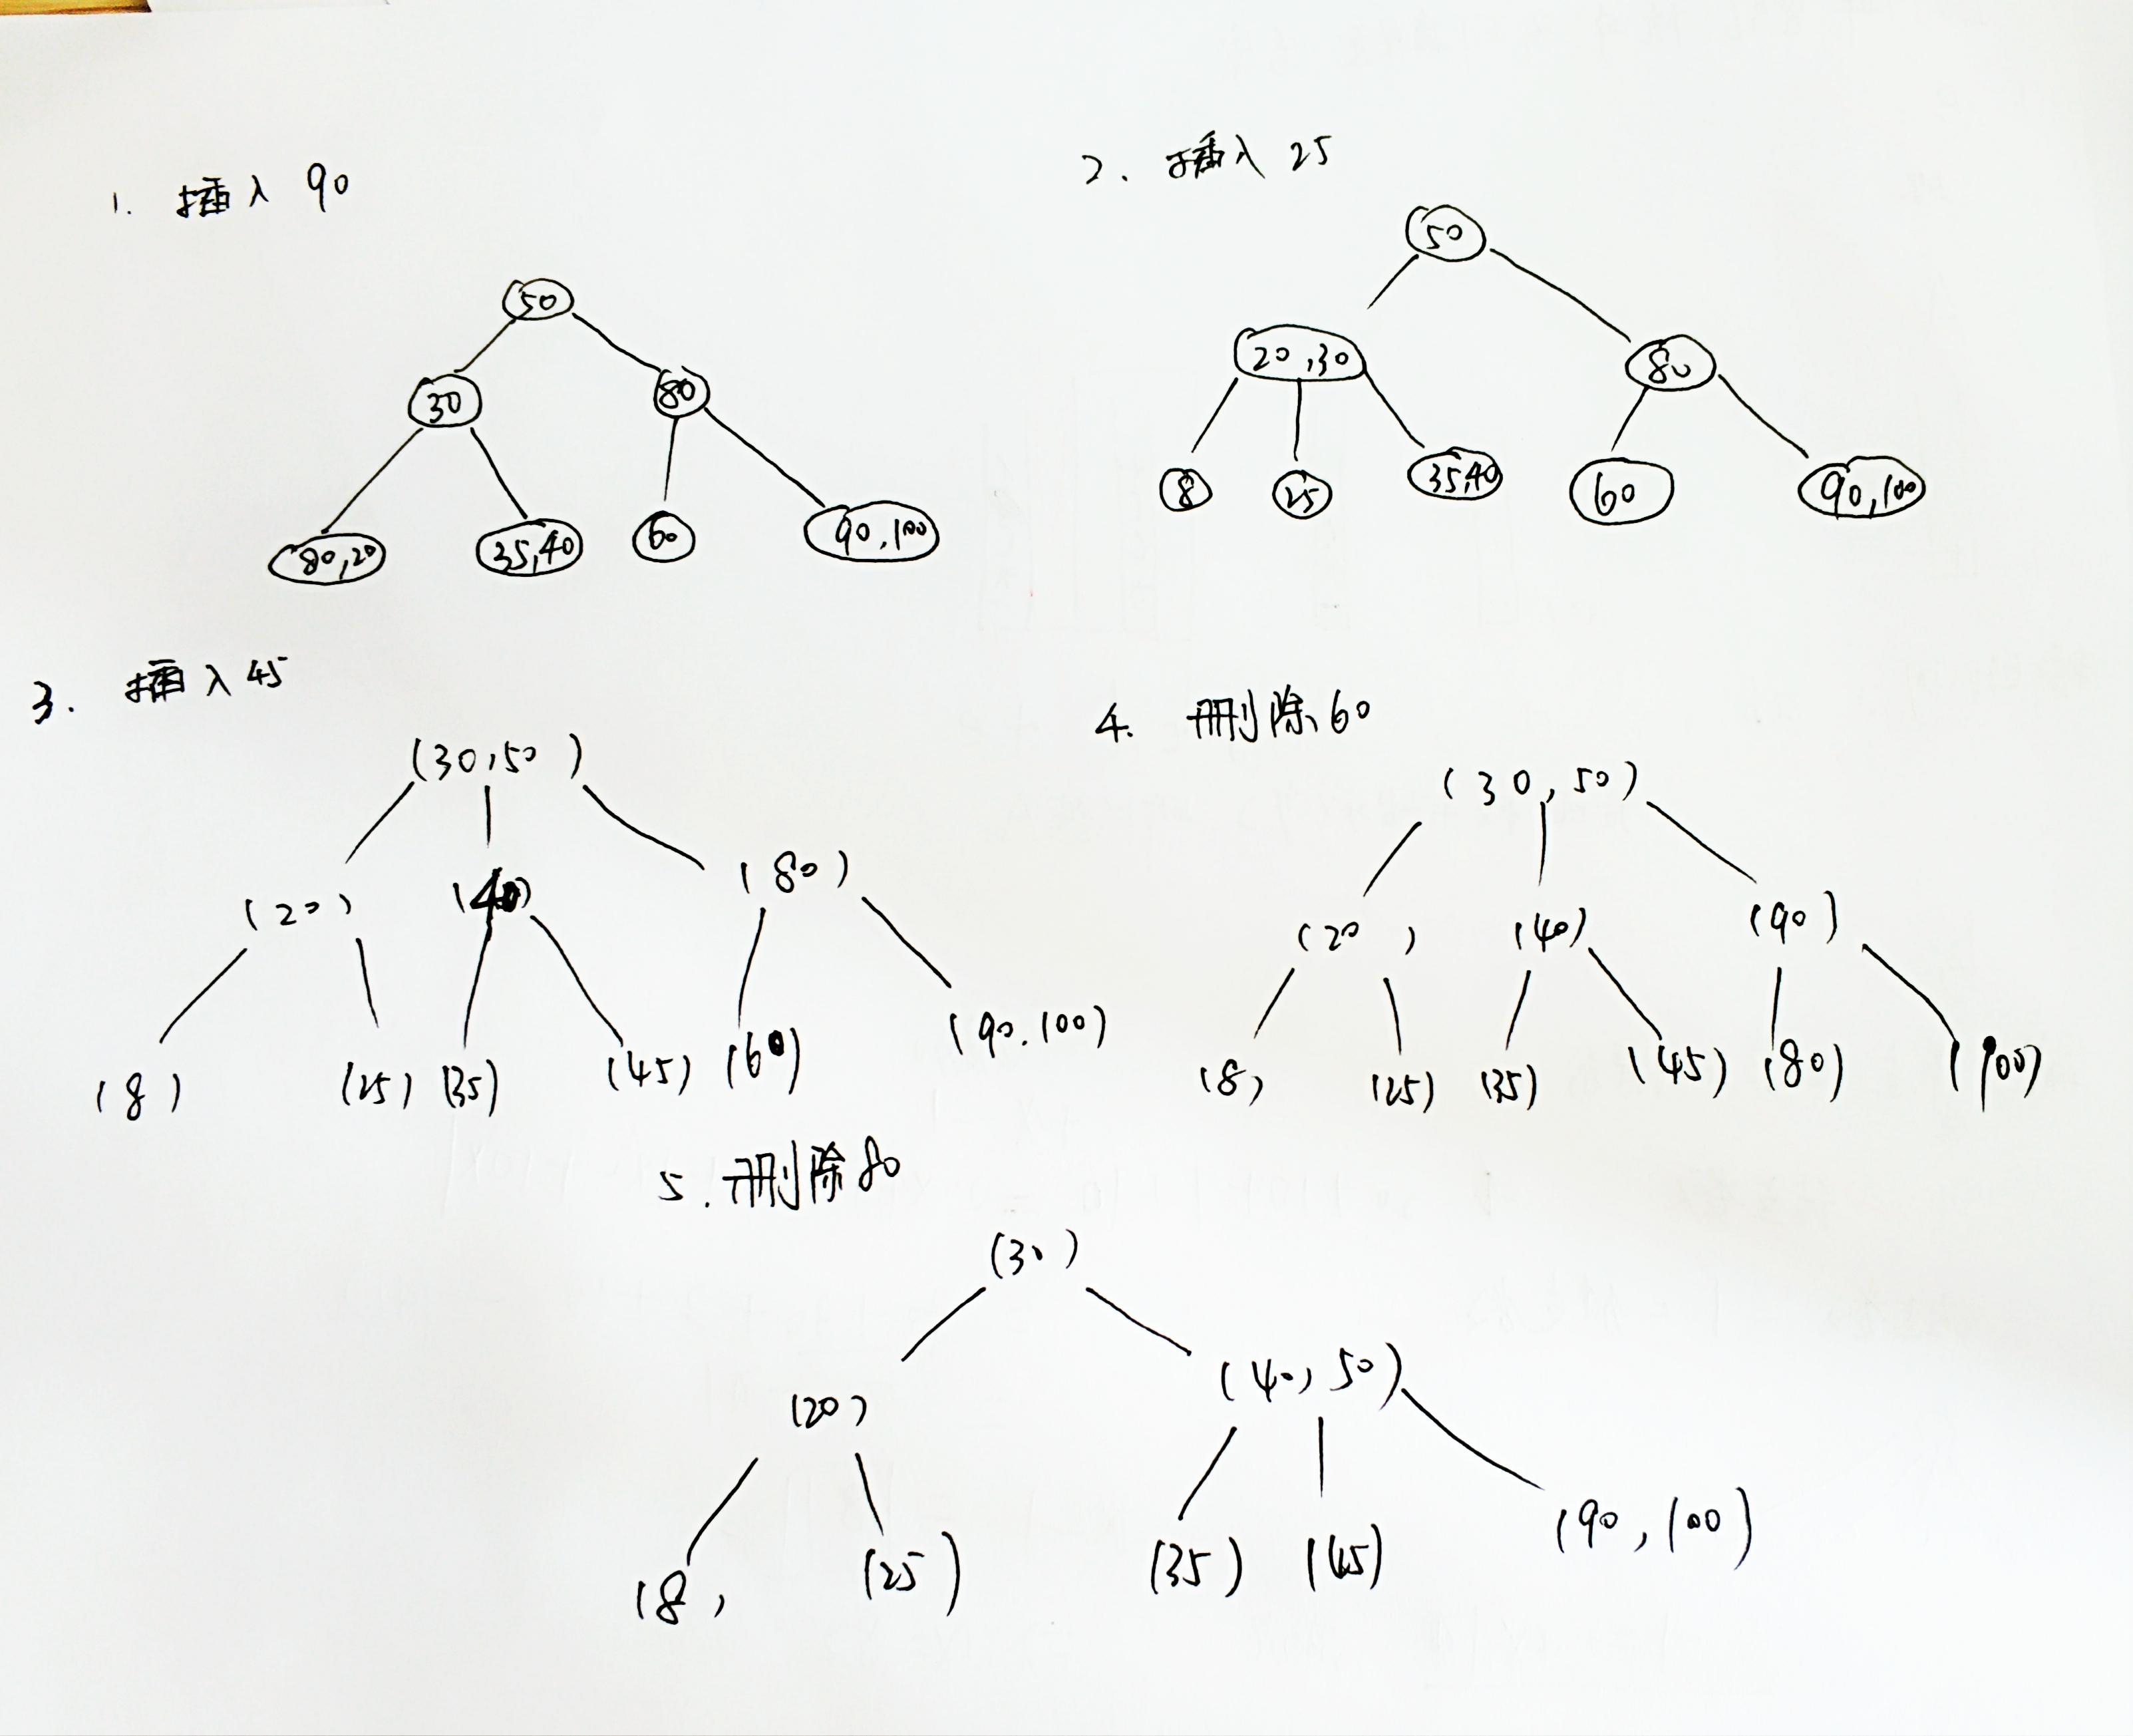
\includegraphics[scale=0.1]{example/chapter23/QQ20190928105701.jpg}
\end{figure}

4. 下标给出了某工程各工序之间的优先关系和各工序所需时间.\newline
\begin{figure}[H]
	\centering  % 环境中的内容居中排版
	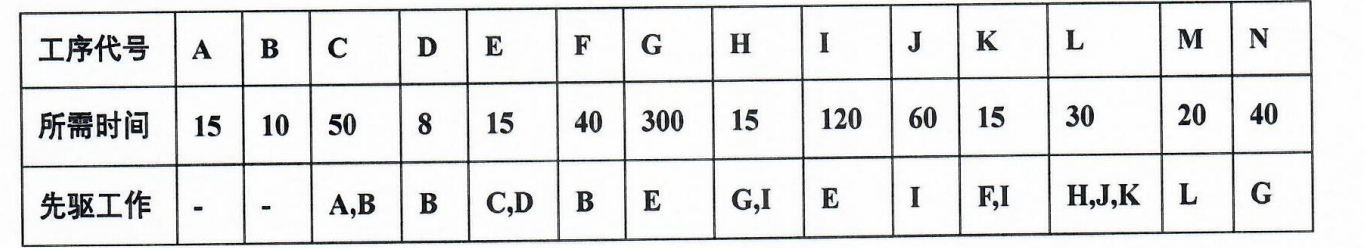
\includegraphics[scale=0.3]{example/chapter23/Annotation2019-09-21144810.png}
\end{figure}
(1) 画出相应的AOE网;\newline
(2) 列出各时间的最早发生时间,最迟发生时间;\newline
(3) 找出关键路径并指明完成该工程所需最短时间.\newline
解:\newline
错题=.=\newline


\subsection{四、程序阅读题(本大题共3小题, 每小题5分, 本大题共15分)}
1. 算法一:\newline
判断是否是连通图\newline

2. 算法二:\newline
合并两个有序序列,从小到大\newline

3. 算法三:\newline
最大的排在最后,第二大的排在最前,以此类推,直到low == high\newline

\subsection{五、算法设计题(本大题共2小题,每小题11分, 本大题共22分)}
1. \newline
算法思想:\newline
首先:\newline
(1)如果p1的指数比p2的指数大的话,新生成一个结点赋以p1的值。p1向后移动一个结点\newline
(2)如果p1的指数比p2的指数相等的话,判断系数项相加是否等于0,如果不等于那么将p1的系数和p2的系数和赋给新的结点,p1和p2都向后移动\newline
(3)如果p2的指数比p1的指数大的话,新生成一个结点赋以p2的值。p2向后移动一个结点\newline
直到p1或p2走到了链的结尾。\newline
然后将剩下的链表赋给新的链表\newline

\begin{lstlisting}[basicstyle=\small\ttfamily, caption={}, numbers=none]
#include <iostream>
using namespace std;
struct PolyNode {
	int coef;
	int expon;
	struct PolyNode *link;
};
typedef struct PolyNode* Polynomial;
Polynomial add(Polynomial a, Polynomial b) {
	Polynomial q = NULL;
	Polynomial head = q;
	while (a && b) {
		if (a->expon > b->expon) {
			Polynomial p = (Polynomial)malloc(sizeof(struct PolyNode));
			p->link = NULL;
			p->coef = a->coef;
			p->expon = a->expon;
			if (q == NULL) {
				q = p; head = q;
			}
			else {
				q->link = p;
				q = p;
			}
			a = a->link;
		}
		else if (a->expon == b->expon) {
			//int expon = a->expon;
			int coef = a->coef + b->coef;
			if (coef != 0) {
				Polynomial p = (Polynomial)malloc(sizeof(struct PolyNode));
				p->link = NULL;
				p->coef = coef;
				p->expon = a->expon;
				if (q == NULL) {
					q = p; head = q;
				}
				else {
					q->link = p;
					q = p;
				}
			}
			a = a->link;
			b = b->link;
		}
		else {
			Polynomial p = (Polynomial)malloc(sizeof(struct PolyNode));
			p->link = NULL;
			p->coef = b->coef;
			p->expon = b->expon;
			if (q == NULL) {
				q = p; head = q;
			}
			else {
				q->link = p;
				q = p;
			}
			b = b->link;
		}
	}
	while (a) {
		Polynomial p = (Polynomial)malloc(sizeof(struct PolyNode));
		p->link = NULL;
		p->coef = a->coef;
		p->expon = a->expon;
		q->link = p;
		q = p;
		a = a->link;
	}
	while (b) {
		Polynomial p = (Polynomial)malloc(sizeof(struct PolyNode));
		p->link = NULL;
		p->coef = a->coef;
		p->expon = a->expon;
		q->link = p;
		q = p;
		b = b->link;
	}
	return head;
}
int main() {
	Polynomial p1 = (Polynomial)malloc(sizeof(struct PolyNode));
	Polynomial p1_1 = (Polynomial)malloc(sizeof(struct PolyNode));
	Polynomial p1_2 = (Polynomial)malloc(sizeof(struct PolyNode));
	Polynomial p2 = (Polynomial)malloc(sizeof(struct PolyNode));
	Polynomial p2_1 = (Polynomial)malloc(sizeof(struct PolyNode));

	p1->coef = 3; p1->expon = 3; p1->link = p1_1;
	p1_1->coef = 5; p1_1->expon = 1; p1_1->link = p1_2;
	p1_2->coef = 6; p1_2->expon = 0; p1_2->link = NULL;

	p2->coef = 3; p2->expon = 2; p2->link = p2_1;
	p2_1->coef = 4; p2_1->expon = 1; p2_1->link = NULL;

	Polynomial out = add(p1, p2);
	while (out!=NULL) {
		cout << out->coef << " " << out->expon << endl;
		out = out->link;
	}

	system("pause");
}
\end{lstlisting}

2.\newline

解:\newline
算法思想:\newline
判断两个结点是否相同\newline
如果T1的左孩子 == T2的左孩子 || T1的左孩子 == T2的右孩子,递归判断剩下的结点是否满足同构\newline
如果T1的右孩子 == T2的左孩子 || T1的右孩子 == T2的右孩子,递归判断剩下的结点是否满足同构\newline
\begin{lstlisting}[basicstyle=\small\ttfamily, caption={}, numbers=none]
#include <iostream>
#include <set>
using namespace std;

#define MaxTree 10
#define ElementType char
#define Tree int
#define Null -1
struct TreeNode {
	ElementType Element;
	Tree Left;
	Tree Right;
}T1[MaxTree], T2[MaxTree];

bool check(int t1, int t2) {//t1 t2 乃 下标
	if (t1 == -1 && t2 == -1) {
		return true;
	}
	if (t1 == -1 || t2 == -1) {
		return false;
	}
	if (T1[t1].Element != T2[t2].Element) {
		return false;
	}

	bool checked = true;
	if (T1[t1].Left == T2[t2].Left) {
		checked = check(T1[t1].Left, T2[t2].Left);
	}
	else if (T1[t1].Left == T2[t2].Right) {
		checked = check(T1[t1].Left, T2[t2].Right);
	}
	else {
		return false;
	}

	if (checked == false) {
		return false;
	}

	if (T1[t1].Right == T2[t2].Left) {
		checked = check(T1[t1].Right, T2[t2].Left);
	}
	else if (T1[t1].Right == T2[t2].Right) {
		checked = check(T1[t1].Right, T2[t2].Right);
	}
	else {
		return false;
	}

	if (checked == false){
		return false;
	}
	return true;
}
int main() {
	for (int i = 0; i < 5; i++) {
		T1[i].Element = 'A' + i;
		T2[i].Element = 'A' + i;
	}
	T1[0].Left = 1;  T1[0].Right = 2;
	T1[1].Left = 3;  T1[1].Right = 4;
	T1[2].Left = -1; T1[2].Right = -1;
	T1[3].Left = -1; T1[3].Right = -1;
	T1[4].Left = -1; T1[4].Right = -1;

	T2[0].Left = 2; T2[0].Right = 1;
	T2[1].Left = 4; T2[1].Right = 3;
	T2[2].Left = -1; T2[2].Right = -1;
	T2[3].Left = -1; T2[3].Right = -1;
	T2[4].Left = -1; T2[4].Right = -1;
	// test
	//T1[1].Element = 'P';
	cout << check(0, 0) << endl;
	system("pause");
}
\end{lstlisting}

\subsection{六、计算题(本大题共3小题,本大题共10分)}
1.\newline
$[x]_{\mbox{原码}} = 0.1101 \times 2^{-2}$\newline
$[x]_{\mbox{阶移}} = 0,11110$\newline
$[x]_{\mbox{规}} = 0,11110;0,110100000$\newline
2.\newline
(教材81页)尾数决定了有效数值的精度\newline
本题,小数点后有9位,则精度为$2^{-9}$\newline
小知识点(P82):对于原码来说,规格化尾数的格式为x.1xxxx,即小数点后第一位(数值最高位)应为1;对于补码来说,规格化尾数的格式为0.1xxxx、1.0xxxxx,即符号位和数值最高位应相反\newline


3.\newline
(浮点数加减,P138)\newline
大端模式:低地址内存存储的是数据的高字节\newline
x=FD50H,y=FAA0H\newline
$[x]_{\mbox{浮}}=1111 1101 0101 0000$\newline
$[Ex]_{\mbox{移}}=1,11111$\newline
$[Mx]_{\mbox{补}}=0.101010000$\newline
$[y]_{\mbox{浮}}=1111 1010 1010 0000$\newline
$[Ey]_{\mbox{移}}=1,11110$\newline
$[My]_{\mbox{补}}=1.010100000$\newline
对阶 Ex-Ey=1,使$[Ey]_{\mbox{移}}=[Ex]_{\mbox{移}}=1,11111$,\newline
同时y的尾数右移一位,$[My]_{\mbox{补}}=1.101010000(0)$\newline
尾数相加减 $[Mx-My]_{\mbox{补}}=[Mx]_{\mbox{补}}+[-My]_{\mbox{补}}$\newline
$[-My]_{\mbox{补}}=0,010110000(0)$\newline
双符号位\newline
[Mx]补   00,101010000\newline
+[My]补  00,010110000(0)\newline
=        01,000000000(0)\newline
双符号为为01,有溢出,需要右规一位,阶码加一,而$[E]_{\mbox{移}}=1,11111$,也溢出,所以浮点数x+y溢出\newline

\subsection{七、设计题(本大题共2小题,本大题共10分)}
1.\newline
解:\newline
2片8k*8b的ROM从2000H开始,1片8k*16b的SRAM从8000H开始\newline
地址需要13位\newline
A15\_\_\_\_\_\_\_\_\_\_\_\_A0\newline
0010 0000 0000 0000\newline
0011 1111 1111 1111    第一片ROM,高三位 001,对应片选信号为y1\newline
0100 0000 0000 0000\newline
0101 1111 1111 1111    第二片ROM,高三位 010,对应片选信号为y2\newline
1000 0000 0000 0000\newline
1001 1111 1111 1111\newline
1010 0000 0000 0000\newline
1011 1111 1111 1111    SRAM对应高三位有两个,100,101,所以对应片选信号有y4和y5,又低电频有效,所以在y4、y5后添加一个与门,只要有一个有效(即为0),就选中SRAM\newline
本题错误就在于片选信号\newline
\begin{figure}[H]
	\centering  % 环境中的内容居中排版
	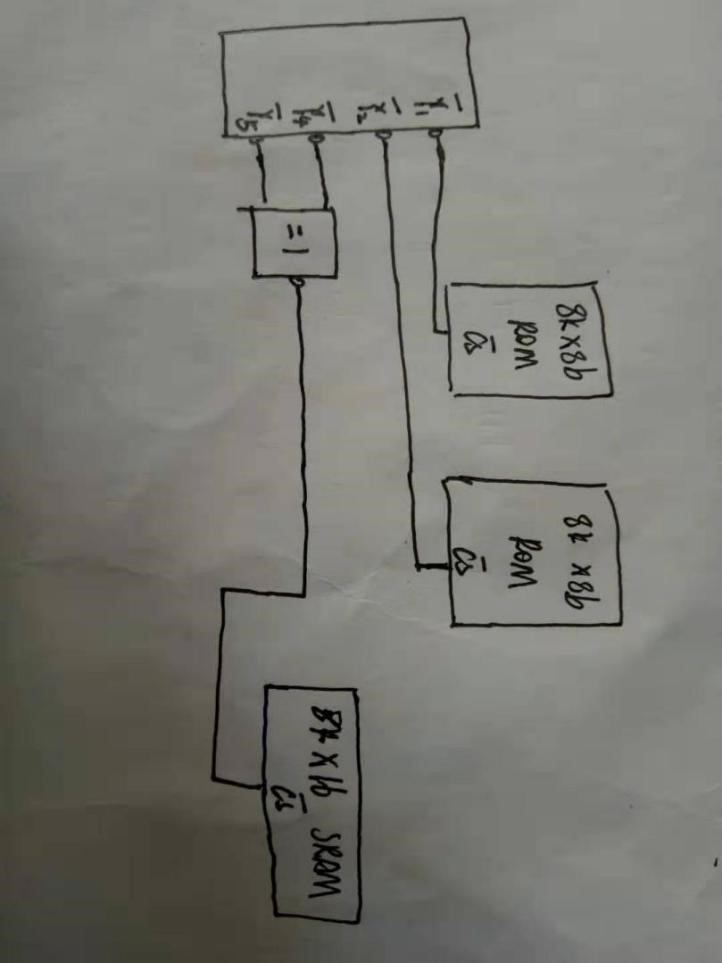
\includegraphics[angle=90]{example/chapter23/dati.jpg}
\end{figure}
2.\newline
应使用多体交叉存储器的方式来最大限度提高带宽\newline
1M*32b/256kB=4*4\newline
共需要16片芯片,分为4组,每组4片,组内进行位扩展\newline
然后构造4个存储体,同一体内地址不连续\newline
(交叉存储器的知识 教材P190)\newline
1M*32b=$2^20$*32b,主存中有$2^20$个单元,主存地址为20位\newline
低2位用于选择存储体,高18位是存储单元在存储体内的相对地址\newline

\subsection{八、(本大题共10分)} 
1. \newline
JNZ LOOP指令起始地址0CH\newline
在执行JNZ LOOP指令时,PC中内容为0EH\newline
偏移 x 14+x=6,x=-8,用补码表示\newline
偏移量 11111000\newline
2. \newline
前一个是寄存器寻址,后一个是变址寻址\newline
3. \newline
8/2=4,该cache中一共有四块,每块正好存放一条指令\newline
前三条指令未命中,3*2=6次\newline
到循环,第一次循环四条指令均未命中,4*2=8次\newline
一共循环10次,剩下9次均命中,4*2*9=72次\newline
最后一条停机指令,未命中2*1=2次\newline
命中率:4*2*9/(3*2+4*2+4*2*9+2*1)*100\%=81.82\%\newline
4. \newline
解:\newline
由上可知,该程序一共未命中16次,命中72次\newline
t=72*10ns+16*(100ns+10ns)=2480ns
\subsection{九、(本大题共15分)}
1. \newline

解:\newline
\begin{tabular}{|c|c|c|c|c|c|c|}% 通过添加 | 来表示是否需要绘制竖线
	\hline  % 在表格最上方绘制横线
	指令 & rd\_rt\_s & imm\_s & rt\_imm\_s  & Alu\_mem\_s	 & Write\_reg & Mem\_Write \\
	\hline % 在表格最下方绘制横线
	ANDi &	1 &	1 &	1 & 1 &	1 &	0 \\
	\hline
\end{tabular}\newline
2. \newline
解:\newline
在这一指令周期内指令不会发生变化 \newline
3. \newline
解:\newline
不能,该指令需要对pc进行修改即pc=pc+offset,该图中没有结构可以实现该运算 \newline
4. \newline
解:\newline
79FBH最高位为0,进行0扩展,得到000079FBH\newline
9F69H最高位为1,进行1扩展,得到FFFF9F69H\newline
5.  \newline
解:\newline
图2的体系结构是哈佛结构,因为数据和指令分开存放\newline
每执行一条指令,pc值+4\newline
6. \newline
解:\newline
属于SISD(教材p12  Flynn分类)\newline